Generally neutrons are born at energies on the order of a few MeV, which is several orders of magnitude above thermal energies.
These neutrons than interact with other nuclei in the material, governed by the probability of a particular reaction occurring.
The probability of a nuclear reaction can be expressed as probable reaction rate for $n$ neutrons traveling with velocity $v$ a distance $x$ in a material with an atomic density of $N$.
This quantity is  defined as the microscopic cross section, $\sigma$, and is expressed in \eqref{eqn:microXS} .
This also gives rise to the macroscopic cross section, $\Sigma=N\sigma$, where the interpretation is the probability per unit path length of the process described by the microscopic cross section \cite{stacey_nuclear_2001}.
\begin{align}
	\label{eqn:microXS}
	\sigma \equiv \frac{\text{reaction rate}}{nvNx}
\end{align}
If the total cross section is known, the mean free path of the neutron can be calculated as $1/\Sigma_\text{tot}$.
In polyethylene, a common neutron moderator, the mean free path of a thermal neutron is about \SI{3.7}{\mm}, and decreases with the addition of strongly absorbing material.
The collisions in the material causes a neutron to lose energy until they thermalized and their energies are on the scale of the temperature of their environment.
For a neutron in thermal equilibrium at \SI{20}{\degreeCelsius} its energy is \SI{0.025}{\eV} and speed is \SI{2000}{\m\per\second}.
In pure hydrogen it takes 27 elastic collisions for a \SI{2}{\MeV} neutron to slow down to \SI{0.025}{\electronvolt}, and 119 collisions in carbon.

In addition to scattering, there are several other reactions that a neutron may undergo in a detector, the most important of these being absorption.
In an absorption reaction the nuclei absorbs the neutron creating a compound nuclei, which is energetically unstable and may release the excess energy by emitting photons or by fissioning.
If the compound nuclei fissions the energy emitted in the reaction (Q-value) is released as the kinetic energy of the fission products.
Several nuclear interactions that are of interest for radiation portal monitors are presented in \autoref{tab:NeutronRxnProducts}.
\begin{table}
	\caption[Neutron Reactions and Reaction Energies]{Typically isotopes used in neutron radiation detectors}
	\label{tab:NeutronRxnProducts}
	\centering
	\begin{tabular}{ m{4cm} | m{1.5cm} m{1.5cm} p{5.5cm}} 
		\toprule
		Reaction                           & Q-Value (MeV) & Thermal Cross Section & Application \\
		\midrule
		${}^3He + n \to p +{}^3H$          & 0.756     & 5,330 & Proportional counter gas \\
		${}^6Li + n \to {}^3H + \alpha$    & 4.78      & 940 & Lithium glass scintillators \\
		${}^{10}B + n \to \alpha + {}^7Li$ & 2.31      & 3,840 & Plastic scintillators \\
		${}^{157}Gd + n \to \gamma$        &various    & 259,000 & various \\
		\bottomrule
	\end{tabular}
\end{table}
The dependance of the cross section on the energy of the neutron is shown in \autoref{fig:NeutronXS}.
The desire to thermalize the neutron flux (decreasing the average energy of the neutrons) is evident due to the dramatic increases of the cross sections for lower energies.
\begin{figure}
	\centering
	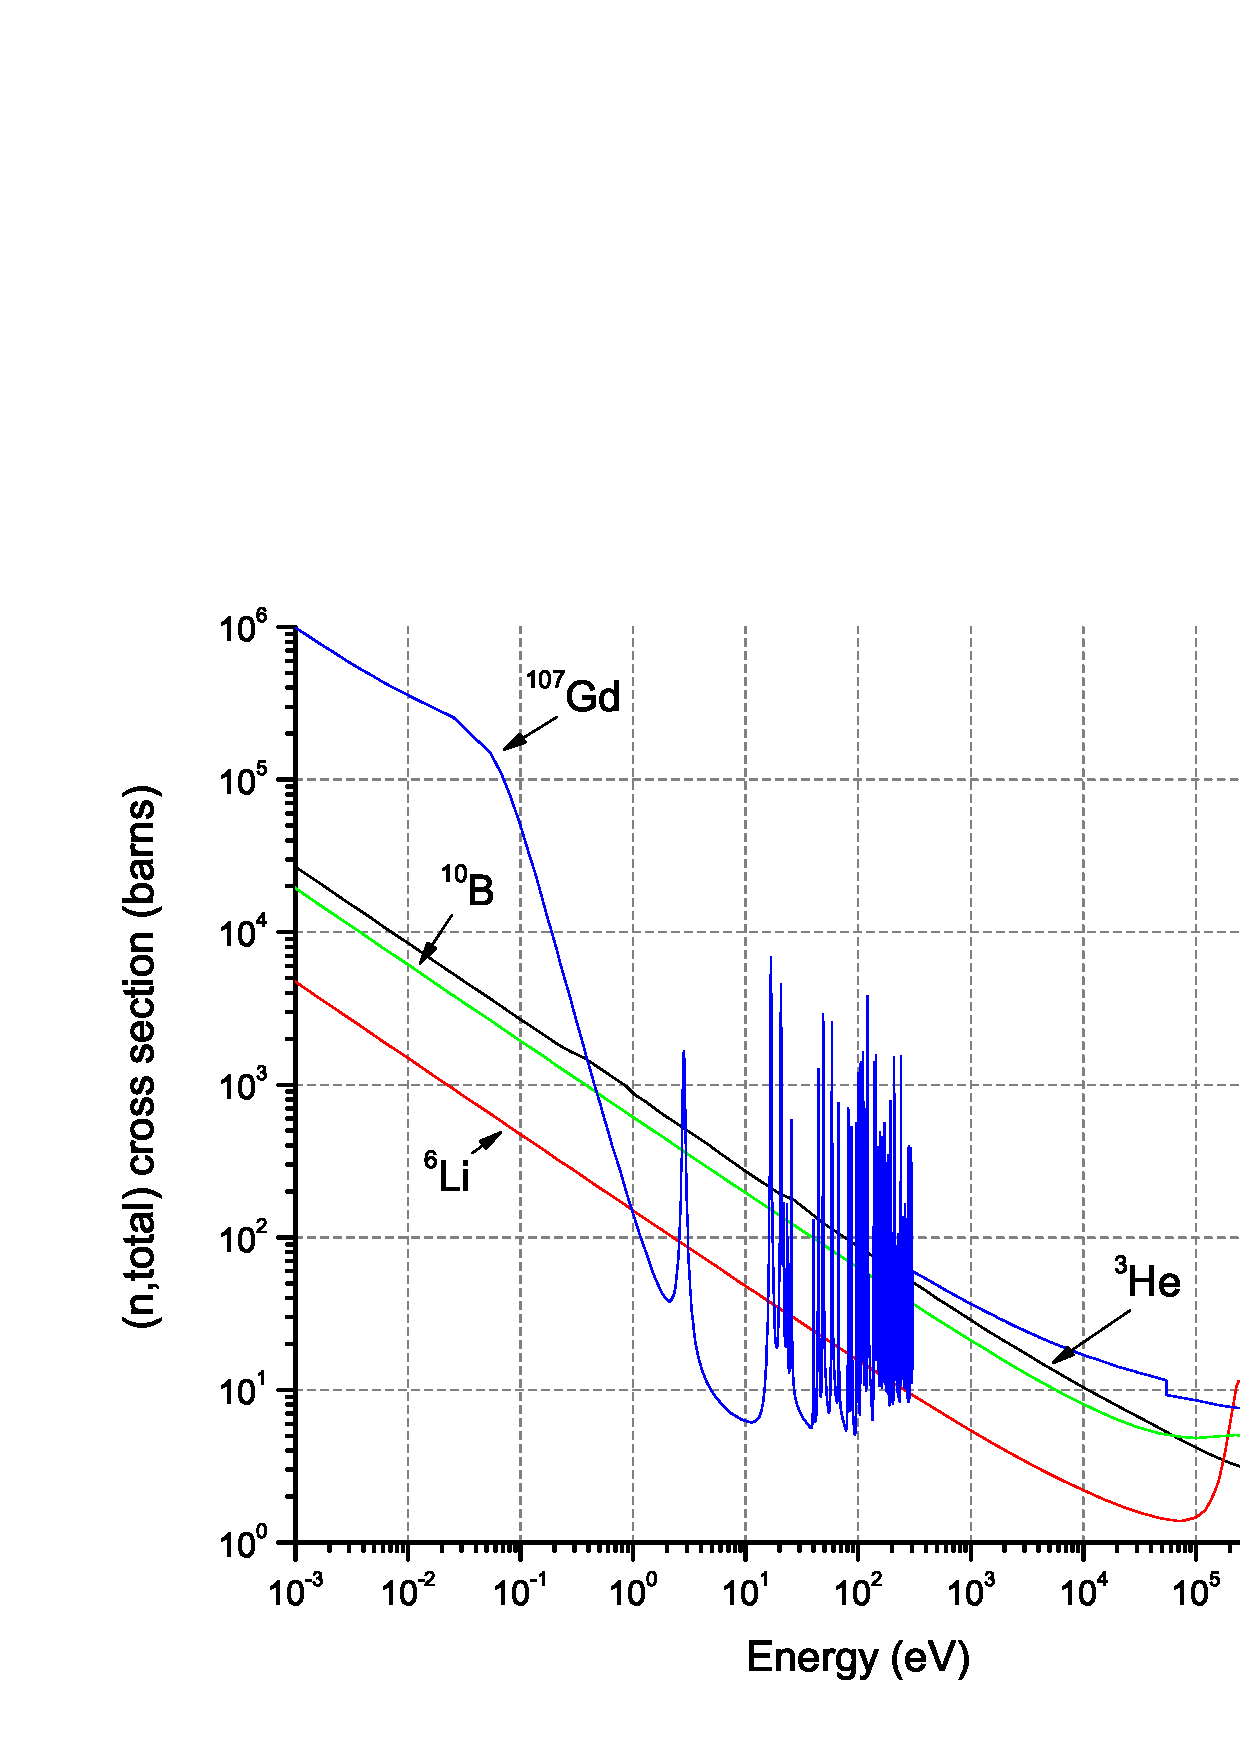
\includegraphics[width=\textwidth]{NeutronXS}
	\caption[Neutron Reaction Cross Sections]{Cross sections of typical isotopes used in neutron radiation detectors.  Neutrons at room temperature have an energy of \SI{0.025}{\eV}.Data from \cite{nndc_cross_2013}.}
	\label{fig:NeutronXS}
\end{figure}
